\documentclass{bcsj}

% --- パッケージの読み込み ---
\usepackage[dvipdfmx]{graphicx}
\usepackage{amsmath}  % 数式環境に必要
\usepackage{float} % 場所の強制配置
\usepackage{subcaption} % 2枚の図を横に並べる
\usepackage{setspace} % 行間調整
\usepackage{titlesec} % セクションタイトルの調整
\usepackage{indentfirst} % 1段落目の字下げ
\usepackage{enumitem} % 箇条書きの調整
\usepackage{makecell}

% \graphicspath{{output/}}

% --- ここから論文情報を記述 ---

% 日本語情報
\title{状態空間モデルを用いた日本国内\\トラック輸送量の外部要因の定量的把握} 
\author{
  寺嶋風雅%
  \affil{中央大学大学院 理工学研究科}
  \and
  赤羽根悠悟%
  \affil{中央大学理工学部}
  \and
  冬木拓実%
  \affil{中央大学大学院 理工学研究科}
  \and
  樋口知之%
  \affil{中央大学理工学部}
}

% 英語情報
\etitle{Structural Change Analysis of Parcel Delivery Volume in Japan Using State-Space Models} 
\eauthor{
  Fuga Terashima%
  \affil{Graduate School of Science and Engineering, Chuo University}
  \and
  Yugo Akahane%
  \affil{Faculty of Science and Engineering, Chuo University}
  \and
  Takumi Fuyuki%
  \affil{Graduate School of Science and Engineering, Chuo University}
  \and
  Tomoyuki Higuchi%
  \affil{Faculty of Science and Engineering, Chuo University}
}
  
% キーワード (英語で3?6個程度)
\keyword{state-space model, structural change, time series analysis, COVID-19, logistics}

% --- ここまでが論文情報 ---


\begin{document}

\maketitle

\begin{abstract}
本研究は, 状態空間モデルを用いて日本国内の宅配便取扱個数の月次データ（2002年4月～2022年7月）における変動要因の分離と定量化を国内で初めて行った. 
先行研究（赤羽根, 2024）では, SARIMA(Seasonal AutoRegressive Integrated Moving Averag)モデルが採用された. 
SARIMAモデルは, ARIMAモデルに季節周期的な変動を取り入れた手法であり, 
過去のデータと誤差の相関構造を利用して高い予測精度を実現する. 
しかし, このモデルでは運賃値上げやコロナ渦のパンデミックといった外的要因が需要に与えたインパクトを数値として分離・評価するには限界があった. 
そこで本研究では, ローカル線形トレンドと季節性に加え, 2017年における主要各社の宅配便運賃値上げと新型コロナウイルス感染症（COVID-19）のパンデミックを外部イベントとして考慮した
複数の状態空間モデルを構築した. 

客観的指標であるAICを用いたモデル比較の結果, 
コロナ禍の影響を複数のフェーズ（構造変化, 第一波, 2021年の波）に分けて固定係数でモデル化した「フェーズ分けモデル」が最も優れたモデルとして採択された. 
本研究は, 状態空間モデルの柔軟性を活用することで, 複雑な時系列データに潜む複数のイベント効果を, その性質に応じて適切に分離・評価できることを実証した. 
これにより, 物流業界の動向をより正確に把握し, 将来の予測や政策決定に資することが期待される. 
\end{abstract}

\section{はじめに}
近年, 日本の物流業界はEコマース市場の拡大に伴い, その重要性を増している (Morganti et al., 2014).
一方で, 『ラストワンマイル問題』に代表される労働力不足(Elsokkary et al., 2022)や, 燃料費の高騰といった多くの課題に直面しており, 
物流の効率化と持続可能性の向上は喫緊の社会課題となっている. こうした背景から, 物流の動向を正確に把握し, 
その変動要因を理解することは, 事業者および政策決定者にとって極めて重要であり、近年では
物流需要や人員配置の最適化(Alqatawna et al., 2023)に向けた時系列予測の取り組みが進められている (e.g., Alqatawna et al., 2023).
この点に関して, \citet{akahane2024} による先行研究は, 国土交通省の統計から20年分の宅配便取扱個数の月次データを構築し, 
SARIMAモデルを用いてその基本構造を分析した. この研究は, 運賃値上げなどのイベントがトレンドに影響を与えた可能性を示唆するなど, 重要な貢献をなした. 
しかし, 同研究ではイベントの外的要因の分離までは困難であり, 
今後の展望として状態空間モデルの適用を提案していた . 
本研究は, この先行研究の課題と提案を直接引き継ぎ, 状態空間モデルを適用することで, 
トレンドや季節性といった基本成分に加え, 複数の外部イベントが与えた影響を, 
その性質に応じて統計的に分離・定量化することを目的とする. 
本研究で使用したデータの原系列を図 \ref{fig:original_series} に示す. 
\begin{figure}[H]
  \centering
  % TeXファイルからの相対パスを直接, すべて記述する
  \includegraphics[width=0.5\textwidth]{../output/originalseries.png}
  \caption{宅配便取扱個数の原系列}
  \label{fig:original_series}
\end{figure}


\section{分析手法} 
\subsection{使用データ} % ← ここに新しいサブセクションを追加

本研究で使用するデータは, 国土交通省が公表する「交通関係統計資料」から取得した2002年4月から2022年7月までの月次データである. 
先行研究（赤羽根, 2024）において構築されたデータセットを利用した. 
主要な変数と宅配便取扱個数の現系列を表\ref{tab:data_columns}に示す. 

\begin{table}[htbp]
  \centering
  \caption{主要変数一覧}
  \label{tab:data_columns}
  % \resizeboxでtabular環境を囲む
  \resizebox{0.5\textwidth}{!}{%
    \begin{tabular}{ll}
      \hline
      カラム名 & 内容 \\
      \hline
      \texttt{label} & 年月 (YYYY-MM-DD) \\
      \texttt{year} & 年 \\
      \texttt{month} & 月 \\
      \texttt{Transport\_tonnage} & 輸送トン数（トン） \\
      \texttt{number\_parcels} & 宅配便取扱個数（千個） \\
      \texttt{Number\_companies\_1} & 輸送トン数の調査会社数（社） \\
      \texttt{Number\_companies\_2} & 宅配便取扱個数の調査会社数（社） \\
      \hline
    \end{tabular}%
  }
\end{table}

変動を安定させるため, 本分析の目的変数には, \texttt{number\_parcels}の自然対数を取った値を用いた.
\subsection{分析モデル}
本研究で用いた状態空間モデル(国友, 1985 ; Kitagawa, 2005)は, 以下のシステムモデルおよび観測モデルによって表現される. 

\begin{align}
    x_t &= F_t x_{t-1} + G_t \eta_{t} \label{eq:system_model} \\
    y_t &= H_t x_t + \beta d_t + \epsilon_t \label{eq:observation_model}
\end{align}

各攪乱項は, 互いに独立な正規分布に従うと仮定する. 
\begin{align}
    \eta_t &=
    \begin{bmatrix}
      \eta_{\mu,t}  \\ % トレンド（レベル）ノイズ
      \eta_{\delta,t} \\ % トレンド（傾き）ノイズ
      \eta_{\gamma,t}  % 季節ノイズ
    \end{bmatrix}
    \sim N \left( 0, 
    \begin{bmatrix}
      \sigma_{\mu}^2 & 0 & 0 \\
      0 & \sigma_{\delta}^2 & 0 \\
      0 & 0 & \sigma_{\gamma}^2
    \end{bmatrix} \right) \label{eq:eta_dist} \\
    \epsilon_t &\sim N( 0, \sigma_{\epsilon}^2) \label{eq:epsilon_dist}
\end{align}

ここで, 状態ベクトル$x_t$は, トレンド成分と周期12の季節成分から構成される. 
具体的には, 状態ベクトル$x_t$, 遷移行列$F_t$, 観測ベクトル$H_t$は, それぞれ以下のように定義される. 

% ↓ ここからが具体的な行列の定義
\begin{align}
    x_t &= 
    \begin{bmatrix}
        \mu_t \\      % トレンドの水準
        \delta_t \\    % トレンドの傾き
        \gamma_t \\    % 現在の季節効果
        \gamma_{t-1} \\ % 過去の季節効果1
        \vdots \\
        \gamma_{t-11}  % 過去の季節効果10
    \end{bmatrix}
    , \\ % 改行したい場所に\\を置く
    F_t &= 
    \begin{bmatrix}
        1 & 1 & 0 & \dots & \dots & 0 \\
        0 & 1 & 0 & \dots & \dots & 0 \\
        0 & 0 & -1 & \dots & \dots & -1 \\
        0 & 0 & 1 & 0 & \dots & 0 \\
        \vdots & \vdots & & \ddots & \ddots & \vdots \\
        0 & 0 & 0 & \dots & 1 & 0
    \end{bmatrix}
    , \\
    H_t &= 
    \begin{bmatrix}
        1 & 0 & 1 & 0 & \dots & 0
    \end{bmatrix}
\end{align}

ここで, $\mu_t$ は $t$ 時点のトレンドの水準, $\delta_t$ はトレンドの傾きを表す. 
$\gamma_t$ は現在の季節効果を示し, 遷移行列 $F_t$ の3行目（$-1, \dots, -1$）により, $\sum_{j=0}^{11} \gamma_{t-j} = 0$ という制約が課される. 
モデルのパラメータ（分散 $\sigma^2$群および係数 $\beta$群）は, 最尤法によって推定される. 

観測方程式 \eqref{eq:observation_model} における外生変数項 $\beta d_t$ は, 運賃値上げおよびコロナ禍の各フェーズが与える影響の総和を表す. 
係数ベクトル $\beta$ および ダミー変数ベクトル $d_t$ は, 具体的に以下のように定義される. 

{
\small % 数式全体を少し小さくする（必要なければ削除可）
\begingroup
\setlength{\arraycolsep}{1.5pt} % 行列の列間隔を詰める（通常は5pt程度）
\begin{align}
    \beta &= 
    \begin{bmatrix}
        \beta_{\mathrm{hike}} & \beta_{\mathrm{covid\_main}} & \beta_{\mathrm{covid\_wave1}} & \beta_{\mathrm{covid\_2021}}
    \end{bmatrix} 
    \label{eq:beta_def} \\
    d_t &= 
    \begin{bmatrix}
        d_{\mathrm{hike}, t} & d_{\mathrm{covid\_main}, t} & d_{\mathrm{covid\_wave1}, t} & d_{\mathrm{covid\_2021}, t}
    \end{bmatrix}^T
    \label{eq:d_def}
\end{align}
\endgroup
}
外生変数項はこれらの内積 $\beta d_t$ として定義される.

\subsection{外生変数の設計}
本研究で用いる状態空間モデルは, トレンドや季節性といった内部構造に加え, 外部からのイベントが時系列に与える影響を分離して分析できる点が特徴である. 
ここでは, 観測方程式に組み込む外生変数$d_t$
 の具体的な設計について述べる. 

宅配便の取扱個数は, 社会・経済情勢の変化に敏感に反応すると考えられる. 
特に, 分析対象期間中には, 業界全体に影響を及ぼした大規模な運賃値上げと, 
人々の生活様式を大きく変容させた新型コロナウイルス感染症（COVID-19）のパンデミックという2つの重要なイベントが発生した. 
これらの影響を適切にモデル化するため, 本研究ではイベントの性質に応じて期間を設定したダミー変数を設計し, 外生変数として導入する. 
各ダミー変数は, イベントが発生している期間は1, それ以外の期間は0をとるバイナリ変数である. 
モデルは, これらの変数に対する係数$\beta$を推定することで, 各イベントが宅配便取扱個数に与えた瞬間的なインパクトの大きさを定量的に評価する. 
具体的な変数設計はに示す通りである. 
本モデルで外生変数として導入するダミー変数は以下の通りである. 

% description を itemize に変更
\begin{itemize}
    \item \textbf{\texttt{hike\_dummy}}: 2017年10月に実施された主要各社の運賃値上げの影響を捉えるための変数. 
    \textbf{（対象期間: 2017/10 -- 2019/12）}
    主要3社（ヤマト運輸, 佐川急便, 日本郵便）の値上げ実施時期から, コロナ禍の影響が顕在化する直前の期間までを設定した. 

    \item \textbf{\texttt{covid\_main}}: COVID-19パンデミックによる巣ごもり需要の定着など, 市場構造そのものに与えた持続的な変化（構造変化）を捉える変数. 
    \textbf{（対象期間: 2020/03 -- ）}
    WHOによるパンデミック宣言や国内での影響が本格化した時期から, 分析期間の終わりまで持続するベースラインの上昇として設定した. 

    \item \textbf{\texttt{covid\_wave1}}: パンデミック初期の短期的なインパクトを捉える変数. 
    \textbf{（対象期間: 2020/04 -- 2020/05）}
    日本国内で最初の緊急事態宣言が発令された期間と一致させており, 外出自粛に伴う一時的な特需を分離するために設定した. 

    \item \textbf{\texttt{covid\_2021}}: 感染再拡大に伴う断続的な需要増の影響を捉える変数. 
    \textbf{（対象期間: 2021/01 -- 2021/09）}
    2回目および3回目の緊急事態宣言が主要都市に断続的に発令されていた期間（デルタ株の流行期）と概ね一致させて設定した. 
\end{itemize}



\subsection{比較モデル}
本研究で採用する最終モデルの優位性, および各外部イベントが与える影響の重要性を評価するため, 以下の3つの状態空間モデルを構築し, 比較検討を行った. 
各モデルは, 2.2節で述べた基本構造を共有しつつ, 2.3節で設計した外生変数の組み込み方が異なる. 

\begin{itemize}
    \item \textbf{ベースラインモデル}: ローカル線形トレンド成分と季節成分のみで構成されるモデル. 
    外部イベントの影響を一切考慮しない, 最も基本的なモデルであり, 分析の基準点（ベンチマーク）となる. 
    \item \textbf{単純イベントモデル}: ベースラインモデルに加え, 運賃値上げダミーと, 
    コロナ禍の影響を単一のダミー変数（\texttt{covid\_main}）のみで表現したモデル. イベントの影響を単純化した形で評価する. 
    \item \textbf{提案モデル}: ベースラインモデルに加え, 運賃値上げダミーと, 
    コロナ禍の影響をその性質に応じて複数のフェーズに分けたダミー変数群（\texttt{covid\_main}, \texttt{covid\_wave1}, \texttt{covid\_2021}）
    を全て組み込んだ, 本研究における提案モデルである. 
\end{itemize}

これらの3モデルをそれぞれ推定し, モデルの当てはまりの良さを情報量規準AIC(Akaike, 1974)によって評価した. 
その比較結果は次章で詳述する. 
\section{分析結果}

\subsection{予備的検討：STL分解と回帰分析}
本分析に先立ち, 外部イベントの影響に関する予備的な検討として, 
STL分解 (Seasonal-Trend decomposition using Loess; Cleveland et al., 1990) および重回帰分析を用いた検証を行った. 
なお, STL分解における平滑化パラメータ（季節成分およびトレンド成分）の決定にあたっては, 
分解後の残差成分の標準偏差（RMSE）を最小化するグリッドサーチを実施した. 
ここで, 単純にRMSEの最小化のみを目的関数とすると, アルゴリズムはトレンド窓幅を極小化し, 
本来残差に含まれるべき短期的なノイズまでもトレンドとして過剰に吸収してしまい, 過学習する傾向がある.  
そのため, 本分析ではトレンドとして解釈可能な滑らかさを担保するべく, トレンド窓幅に対し「21ヶ月（約2年分）以上」
という明示的な制約条件を課した上で, 最適解を探索・採用した. 
まず, 原系列（対数変換値）をSTL分解によりトレンド, 季節, 残差成分に分離した結果を図\ref{fig:stl_decomp}に示す. 

% --------------------------------------------------
% STL分解の結果図
% --------------------------------------------------
\begin{figure}[H]
  \centering
  \includegraphics[width=\linewidth]{../output/decomposition_STL.png} % 保存したファイル名
  \caption{STL分解による時系列成分の分離}
  \label{fig:stl_decomp}
\end{figure}
次に, この残差成分を目的変数とし, 2.3節で定義した4つのイベントダミー変数 (\texttt{hike\_dummy}, \texttt{covid\_main},
 \texttt{covid\_wave1}, \texttt{covid\_2021}) を説明変数とした重回帰分析を行った. その結果を表\ref{tab:ols_result}に示す. 

% --------------------------------------------------
% 重回帰分析の結果表
% --------------------------------------------------
\begin{table}[H]
  \centering
  \caption{STL分解残差に対する重回帰分析の結果}
  \label{tab:ols_result}
  \footnotesize 
  
  \setlength{\tabcolsep}{6pt} 

  \begin{tabular}{lrrcc}
    \hline
    % ヘッダー
    パラメータ
      & \multicolumn{1}{c}{\makecell{係数 \\ (coef)}} 
      & \multicolumn{1}{c}{\makecell{標準誤差 \\ (std. err)}} 
      & \multicolumn{1}{c}{\makecell{t値 \\ (t-val)}} 
      & \makecell{p値 \\ ($P>|z|$)} \\ % ←短縮
    \hline
    Intercept         &  0.0029 & 0.0016 &  1.850 & 0.066 \\
    \texttt{hike\_dummy} & -0.0060 & 0.0045 & -1.333 & 0.184 \\
    \texttt{covid\_main} &  0.0097 & 0.0054 &  1.801 & 0.073 \\
    \texttt{covid\_wave1}& 0.0667 & 0.0162 & 4.111 & 0.000 \\
    \texttt{covid\_2021} & -0.0091 & 0.0089 & -1.021 & 0.309 \\
    \hline
    \multicolumn{5}{r}{($R^2=0.111, \text{Durbin-Watson}=1.377$)} \\
  \end{tabular}
\end{table}

この結果は, コロナの第一波におけるショックが強力であることを示唆している. 
また, 本回帰モデルのDurbin-Watson比は $1.377$ であった. 
これは, モデルの残差に正の自己相関が残存していることを示しており, 
回帰係数の標準誤差が過小評価され, $t$ 値が見かけ上高く算出されるバイアスが生じている可能性を示唆する. 
したがって, 残差の自己相関構造を適切に処理し, より信頼性の高い推定を行うためには, 次節で導入する状態空間モデルによる分析が必要である. 

\subsection{モデルの比較と選択}
\begin{table}[H]
  \centering
  \caption{モデルの比較}
  \label{tab:model_comparison}
  \small % ← この行を追加
  \begin{tabular}{lccc}
    \hline
    モデル & 対数尤度 & AIC & BIC \\
    \hline
    1. ベースラインモデル & 471.9 & -913.9 & -861.4 \\
    2. 単純イベントモデル & 477.5 & -915.0 & -855.1 \\
    \textbf{3. 提案モデル} & \textbf{480.9} & \textbf{-919.9} & \textbf{-846.4} \\
    \hline
  \end{tabular}
\end{table}

なお, パラメータ数に対しより強いペナルティを課すBICでは, 
よりシンプルな『単純イベントモデル』が最良となった（表2）. 
しかし本研究では, コロナ禍のインパクトをその性質に応じて複数のフェーズに分離して解釈することの理論的な重要性を重視し, 
AICに基づき『提案モデル』を分析対象として採択した. 

\subsection{提案モデルの推定結果}
提案モデルのパラメータ推定結果を表\ref{tab:final_model_params}に示す. 
本研究で提案する状態空間モデルのパラメータ推定には, PythonのライブラリであるStatsmodels (Seabold, Perktold, 2010) を用いた.
具体的には, 同ライブラリの MLEModel クラスを継承して独自のクラスを構築し,
 (2.5)～(2.9)式で定義した遷移行列および観測行列を実装することで,
カルマンフィルタによる対数尤度の計算および最尤推定を行った.
なお, 各モデルのパラメータ推定にあたっては初期値依存を避け安定した解を得るため, 複数の初期値候補によるグリッドサーチによって最尤解を探索した.
\begin{table}[H]
  \centering
  \caption{提案モデルのパラメータ推定結果}
  \label{tab:final_model_params}
  \footnotesize
  % \resizebox を削除
  % ↓ ヘッダーを makecell で改行し, p値を数式モードにする
  \begin{tabular}{lrrc}
    \hline
    パラメータ & \multicolumn{1}{c}{\makecell{推定値 \\ (coef)}} 
             & \multicolumn{1}{c}{\makecell{標準誤差 \\ (std err)}} 
             & \makecell{p値 \\ ($P>|z|$)} \\
    \hline
    \multicolumn{4}{l}{\textit{外生変数効果}} \\
    % ↓ _ を \ (バックスラッシュ) でエスケープする
    \texttt{hike\_effect} & -0.023 & 0.031 & 0.464 \\
    \texttt{covid\_main\_effect} & 0.049 & 0.040 & 0.222 \\
    \texttt{covid\_wave1\_effect} & 0.045 & 0.026 & 0.077 \\
    \texttt{covid\_2021\_effect} & 0.020 & 0.015 & 0.184 \\
    \hline
    \multicolumn{4}{l}{\textit{分散パラメータ}} \\
    観測ノイズ ($\sigma_{\epsilon}^2$) & 0.0003 & 4.35e-05 & 0.000 \\
    トレンドノイズ ($\sigma_{\mu}^2$) & 8.66e-05 & 2.29e-05 & 0.000 \\
    傾きノイズ ($\sigma_{\delta}^2$) & 2.46e-11 & 2.61e-08 & 0.999 \\
    季節ノイズ ($\sigma_{\gamma}^2$) & 5.30e-05 & 1.63e-05 & 0.001 \\
    \hline
  \end{tabular}
  % \resizebox の閉じ括弧も削除
\end{table}

表\ref{tab:final_model_params}から,コロナ禍第一波の効果（\texttt{covid\_wave1\_effect}）の係数が約0.045であり, 10\%水準で統計的に有意であったことが確認できる（p=0.077）. 
これは, 最初の緊急事態宣言下において, 他の要因に加えて約4.5\%の追加的な需要増があったことを示唆している. 
一方で, 2017年の運賃値上げ効果（\texttt{hike\_effect}, p=0.464）や, コロナ禍による持続的な構造変化（\texttt{covid\_main\_effect}, p=0.222）, 2021年の波（\texttt{covid\_2021\_effect}, p=0.184）については, 本モデルでは統計的に有意な水準の変化としては検出されなかった. 
% 統計的に有意だった効果などを文章でハイライトします. 

\subsection{時系列の成分分解}
% ここに, 最終モデルによる分解グラフを載せ, 
% トレンドや季節性, イベント効果がどのように現れているかを視覚的に説明します. 
提案モデルによる分解結果を図\ref{fig:Decomposition_series} に示す. 
\begin{figure}[H]
  \centering
  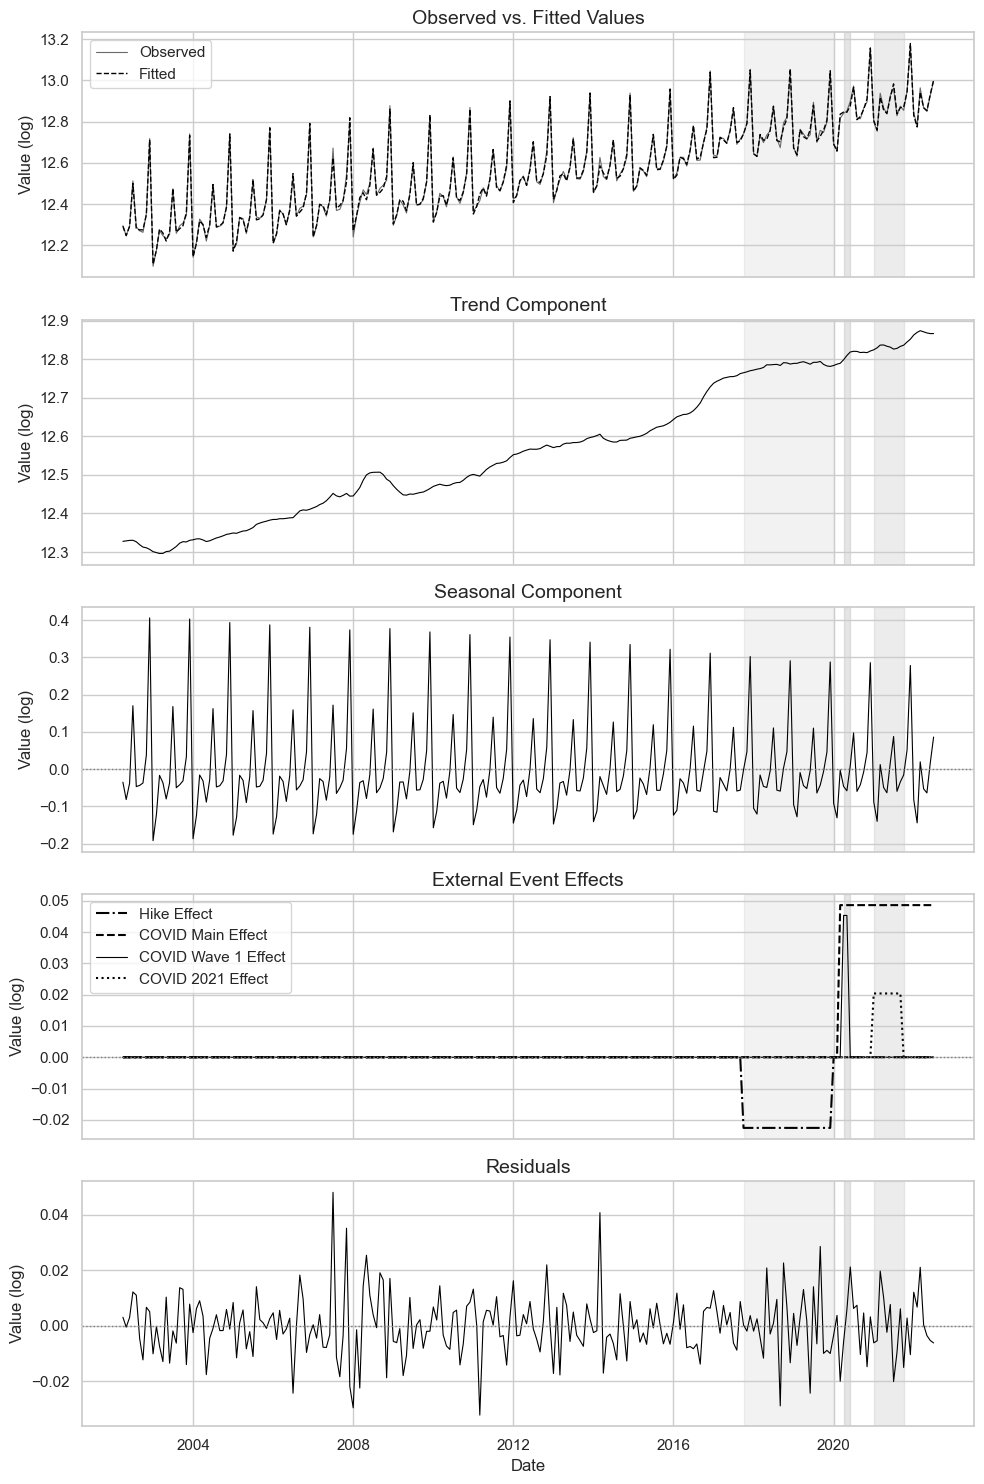
\includegraphics[width=0.5\textwidth]{../output/Decomposition.png}
  \caption{提案モデルによる時系列成分の分解}
  \label{fig:Decomposition_series}
\end{figure}
図\ref{fig:Decomposition_series}上段の観測値とフィット値の比較から, モデルが実際のデータの変動を非常によく捉えていることがわかる. 
中段のトレンド成分は, 分析期間を通して一貫した上昇傾向を示している. 表3のパラメータ推定結果では, 
傾きノイズ（$\sigma_{\delta}^2$）がほぼゼロ（2.46e-11）と推定されており, これはトレンドの成長率が分析期間を通じてほぼ一定であったことを示唆している. 
また, 2007年後半にかけて急激な水準の上昇が確認できる. これは, 2007年10月の日本郵政公社民営化に伴い, 
「ゆうパック」が国土交通省の自動車運送事業統計の集計対象に新たに算入されたことによる, 
統計定義上の構造変化を反映している.  本モデルのトレンド成分は, 
このような外部要因による統計上の不連続な水準変動に対しても, 
確率的な変動として柔軟に追従・適応しており, モデルが高いロバスト性を有していることを示している. 
下段の季節成分は, 毎年夏に減少し冬に増加する, 安定した周期変動を示している. 
上段の外部イベント効果を見ると, コロナ禍第一波の期間に, 他のイベントよりも顕著な正のインパクトが瞬間的に発生していることが視覚的に確認できる. 
下段の残差は, 全体として特定のパターンを持たないランダムな変動となっており, モデルがデータの主要な構造を十分に捉えられていることを示唆している. 

\section{考察}
\subsection{コロナ禍における需要変動の構造的解釈}
本分析が提示する重要な知見は, コロナ禍が宅配便需要に与えたインパクトが, 
単一の現象ではなく「持続的なベースラインの上昇」という構造変化と, 「第一波における短期的な需要急増」
というショックの複合であったと統計的に分離・定量化できた点にある. この複合的な性質の解明は, 
先行研究のSARIMAモデルでは困難であり, 状態空間モデルの優位性を示すものである. 
コロナ禍がサプライチェーン全体に与えた混乱や構造変化については(Vilko, Hallikas, 2024) も指摘しており, 本モデルが捉えたベースラインの上昇は
こうした世界的な傾向とも一致していると考えられる.

\subsection{分析手法の比較とモデルの頑健性}
また, 本研究ではモデルの頑健性を検証するため, 予備的検討としてSTL分解と重回帰分析を用いた比較検証を行った. 
異なるアプローチを用いたが, 両手法ともに
「コロナ禍第一波 (\texttt{covid\_wave1}) のみが統計的に有意な正のインパクトを与え, 
その他のイベント効果は有意ではない」という主要な結論が一致した. 
このことは, 本研究で得られた知見が, 特定のモデル仕様に依存した結果ではなく, データそのものが有する頑健な特性であることを示唆している. 
一方で, 両手法の結果には質的な差異も見られる. 
単純な重回帰分析では \texttt{covid\_main}（構造変化）
の$p$値が $0.073$ と10\%水準で有意に近い値を示したのに対し, 
状態空間モデル（表4）では $0.222$ とより保守的な結果となった. 
重回帰分析におけるDurbin-Watson比 ($1.377$) が示す通り, 単純なモデルでは残差の自己相関を考慮できないため, 
標準誤差が過小評価され, $t$値が見かけ上高く算出されるバイアスが生じやすい. 
これに対し, 状態空間モデルはトレンドや季節性の確率的な変動を明示的にモデル化することで, この自己相関の問題に対処している. 
したがって, 状態空間モデルによる推定結果の方が統計的により信頼性が高く, コロナ禍の長期的な影響については慎重な解釈が必要であることを示している. 

さらに, この結果の差異は, 両手法のアルゴリズム的な性質の違いからも説明できる. 
ここで改めてSTL分解の挙動を整理すると, その本質は局所重み付き回帰（LOESS）を用いて季節とトレンドを交互に更新・平滑化する反復プロセスにある. 
すなわち, STLは分析者が設定したトレンド幅などのパラメータに従って, 決定論的に成分を配分する手続き的アプローチである. 
この手法は探索的なデータ分析（EDA）には有用であるが, パラメータ設定に分析者の恣意性が介入する余地が残り, 
急激なショックが発生した際に, それがトレンドと残差のどちらに吸収されるかが計算ルールに依存するという構造的な課題を持つ. 
対して, 本研究で採用した状態空間モデルは, データの背後にある確率的な生成過程を仮定し, 
尤度に基づいてパラメータを推定するモデルベースのアプローチである. 
この手法では, トレンド自体の揺らぎを確率的に許容できるため, コロナ禍のような外的要因を
分析者の主観的なパラメータ設定ではなく, 尤度という客観的な指標に基づいて評価できる. 
結果として, 状態空間モデルの方がノイズやトレンドの変動をより厳密に分離でき, 
これが外部イベントの影響評価における保守的かつ信頼性の高い結果につながったと解釈できる. 

\subsection{運賃値上げの影響とその他の要因}
さらに, 本モデルは2017年の運賃値上げの影響が, コロナ禍のような巨大な変動を考慮すると統計的に有意でなかったことも示唆した. 
これは, Eコマース市場の拡大という強力な上昇トレンド（図2）によって, 
値上げによる仮に存在したであろう負の効果が相殺され, 統計的に検出できなくなった可能性が考えられる. 
あるいは, そもそも宅配便需要の価格弾力性が低く (Oum et al., 1992; Kaplan et al., 2011), 
値上げ幅が需要全体の変動に比べて小さかった可能性も示唆している.

さらに, イベントの性質による影響メカニズムの違いも明らかになった. 
また, 先行研究（赤羽根, 2024）ではリーマンショック時期のトレンド成長率の鈍化が示唆されたが, 
本モデルの推定結果では, 成長率自体の変化は検出されなかった. 
これは, 先行研究で見られた変動が, 成長率の変化ではなく, 本モデルが捉えた水準への一時的なショックであった可能性を示している. 
コロナ禍は需要水準自体の急激な変化として捉えられ, 状態空間モデルが多様なショックを表現できることを実証した. これは, 
物流需要の動態をより深く理解する上で, 本モデルが強力な分析ツールであることを示している. 

本研究ではコロナ禍を複数のフェーズに分離したが, 統計的に有意であったのは\texttt{covid\_wave1\_effect}のみであり, \texttt{covid\_main}や\texttt{covid\_2021}は有意ではなかった . 
これは, これらの影響が本モデルで仮定した「固定期間での瞬間的な水準変化」という単純な形ではなく, 
トレンドの傾きへの影響や, 徐々に減衰する効果などの複雑な動態を持っていた可能性を示唆している. 
これらの動的な影響を捉えることは, 今後の課題である. 

\section{おわりに}
本研究は, 状態空間モデルを日本の宅配便取扱個数データに適用し, 先行研究のSARIMAモデルでは困難であった外部イベント効果の分離・定量化を試みた. 
その結果, 特にコロナ禍のインパクトが社会構造の変化を反映した持続的な需要の底上げと, 
コロナ禍第一波における短期的な特需という, 複合的な現象である可能性をモデル化し, 特に短期的特需については統計的な有意性（p=0.077）を確認した. 
本研究で得られた知見は, 物流業界が直面する「ラストワンマイル問題」などの経営課題に対し, データに基づいた示唆を与えるものである. 

本モデルが示した持続的な構造変化と短期的なショックの分離は, 
物流事業者の意思決定に直接的な示唆を与える. 前者は配送センターの新設といった長期的な設備投資の根拠となり得る一方, 
後者は短期的な人員配置の最適化や一時的なアウトソーシングの判断材料となる. 
本研究では伝統的なアプローチを採用したが, 
近年ではRamosら(2024)が提唱する「State Space Learning: SSL」という
統計的機械学習を用いたアプローチも登場しており, また深層学習を用いた予測手法 (Lim, Zohren, 2021) や大規模な加法モデル (Taylor, Letham, 2018) の活用も含め, 
今後の応用が考えられる.  


% \begin{acknowledgement}
% \end{acknowledgement}

\begin{thebibliography}{99}
  \setlength{\itemsep}{0pt}

% \bibitem{key} を \bibitem[著者(年)]{key} の形式に変更
% (著者が3名以上の場合は "et al." 

\bibitem[赤羽根(2024)]{akahane2024}
赤羽根 悠悟 (2024). 日本国内におけるトラック輸送量の時系列予測と分析. 中央大学理工学部卒業論文.

\bibitem[北川(2005)]{kitagawa2005}
北川 源四郎 (2005). 時系列解析入門. 岩波書店.

\bibitem[国友(1985)]{kunitomo1985}
国友 直人 (1985). 時系列モデル入門. 東京大学出版会.

% \bibitem[姜(2025)]{kyo2025}
% 姜興起 (2025). 現代 時系列解析: 移動線形モデルの方法と実践. 共立出版.

% AICの論文
\bibitem[Akaike(1974)]{akaike1974}
Akaike, H. (1974). A new look at the statistical model identification. 
\textit{IEEE Transactions on Automatic Control}, 19(6), 716--723.

% \bibitem[Akaike(1980)]{akaike1980}
% Akaike, H. (1980). Likelihood and the Bayes procedure. 
% In Bernardo, J. M. et al. (eds.), \textit{Bayesian Statistics}, University Press, 143--166.

\bibitem[Harvey(1990)]{harvey1990}
Harvey, A. C. (1990). \textit{Forecasting, structural time series models and the Kalman filter}. Cambridge university press.

\bibitem[Seabold \& Perktold(2010)]{seabold2010}
Seabold, S., \& Perktold, J. (2010). Statsmodels: Econometric and statistical modeling with python. 
In \textit{9th Python in Science Conference}.

\bibitem[Alqatawna et al.(2023)]{alqatawna2023}
Alqatawna, A., Abu-Salih, B., Obeid, N., \& Almiani, M. (2023). 
Incorporating time-series forecasting techniques to predict logistics companies' staffing needs and order volume. 
\textit{Computation}, \textit{11}(7), 141.

% \bibitem[Vališ et al.(2017)]{valis2017}
% D. Vališ, D. Mazurkiewicz, and M. Forbelská, 
% "Modelling of a Transport Belt Degradation Using State Space Model,"
% in \textit{IEEE International Conference on Industrial Engineering and Engineering Management (IEEM)}, 2017, pp. 136-140.

% \bibitem[Ghareeb(2023)]{ghareeb2023}
% Ghareeb, A. (2023).
% Time series forecasting of stock price for maritime shipping company in COVID-19 period using multi-step long short-term memory (LSTM) networks.
% In \textit{Proceedings of the 17th International Conference on Business Excellence 2023} (pp. 1728-1747).

\bibitem[Ramos et al.(2024)]{ramos2024}
Ramos, A., Valladão, D., \& Street, A. (2024). 
\textit{Time Series Analysis by State Space Learning}. 
arXiv preprint arXiv:2408.09120.

% 価格弾力性の理論的定義
\bibitem[Kaplan et al.(2011)]{kaplan2011}
Kaplan, U., T{\"u}rkay, M., Karas{\"o}zen, B., \& Biegler, L. T. (2011).
Optimization of supply chain systems with price elasticity of demand.
\textit{INFORMS Journal on Computing}, 23(4), 557-568.

% 価格弾力性の文献
\bibitem[Oum et al.(1992)]{oum1992}
Oum, T. H., Waters, W. G., \& Yong, J. S. (1992).
Concepts of price elasticities of transport demand and recent empirical estimates. 
\textit{Journal of Transport Economics and Policy}, 26(2), 139--154.

% ラストワンマイル問題の文献
\bibitem[Morganti et al.(2014)]{morganti2014}
Morganti, E., Seidel, S., Blanquart, C., Dablanc, L., \& Lenz, B. (2014).
The impact of e-commerce on final deliveries: alternative parcel delivery services in France and Germany.
\textit{Transportation Research Procedia}, 4, 178-190.

\bibitem[Vilko and Hallikas(2024)]{vilko2024}
Vilko, J., \& Hallikas, J. (2024).
Impact of COVID-19 on logistics sector companies.
\textit{International Journal of Industrial Engineering and Operations Management}, 6(1), 25-42.

% 因果推論の文献
\bibitem[Brodersen et al.(2015)]{brodersen2015} 
Brodersen, K. H., Gallusser, F., Koehler, J., Remy, N., Scott, S. L. (2015). 
Inferring causal impact using Bayesian structural time-series models. 
\textit{The Annals of Applied Statistics}, 9(1), 247--274.

% STL分解の論文
\bibitem[Cleveland et al.(1990)]{cleveland1990}
Cleveland, R. B., Cleveland, W. S., McRae, J. E., \& Terpenning, I. (1990).
STL: A seasonal-trend decomposition procedure based on Loess. 
\textit{Journal of Official Statistics}, 6(1), 3--73.

\bibitem[Durbin and Koopman(2012)]{durbin2012}
Durbin, J., \& Koopman, S. J. (2012). 
\textit{Time series analysis by state space methods} (2nd ed.). Oxford University Press.

% Prophetの論文
\bibitem[Taylor and Letham(2018)]{taylor2018}
Taylor, S. J., \& Letham, B. (2018).
Forecasting at scale. 
\textit{The American Statistician}, 72(1), 37--45.

% % 時系列予測の基礎理論
% \bibitem[Hyndman and Athanasopoulos(2021)]{hyndman2021}
% Hyndman, R. J., \& Athanasopoulos, G. (2021). 
% \textit{Forecasting: principles and practice} (3rd ed.).
% OTexts: Melbourne, Australia.

% 物流の課題解決
\bibitem[Wang et al.(2020)]{wang2020}
\bibitem[Elsokkary et al.(2022)]{elsokkary2022}
Elsokkary, N., Otrok, H., Singh, S., Mizouni, R., Barada, H., \& Omar, M. (2022).
Crowdsourced last mile delivery: Collaborative workforce assignment. 
\textit{SSRN Electronic Journal}.

% DLと統計モデルの比較
\bibitem[Lim and Zohren(2021)]{lim2021}
Lim, B., \& Zohren, S. (2021). Time-series forecasting with deep learning: a survey. 
\textit{Philosophical Transactions of the Royal Society A}, 379(2194), 20200209.

\end{thebibliography}

\begin{eabstract}
This study utilizes state-space models (SSMs) to investigate how to separate and quantify the factors
 influencing the monthly volume of parcel deliveries in Japan, using data from April 2002 to July 2022.
  While prior research employed SARIMA models, they faced limitations in isolating and quantifying the impact
   of external events—such as delivery fee hikes and the COVID-19 pandemic—on demand. Therefore,
    this study constructs multiple SSMs that incorporate a local linear trend and seasonality,
     while also accounting for these external events.

Based on model comparisons using the Akaike Information Criterion (AIC),
 a "phased model" was selected for further analysis, as it showed the best fit on this criterion.
  This model treats the impact of the COVID-19 pandemic using fixed coefficients
   divided into multiple phases (e.g., structural change, the first wave, and the 2021 wave).
    This research proposes a framework in which, by leveraging the flexibility of SSMs,
     the effects of multiple events embedded in complex time series data can be appropriately
      separated and evaluated according to their respective characteristics.
       This approach suggests that such modeling can contribute to a more accurate understanding
        of trends in the logistics industry and inform future forecasting and policy-making.
\end{eabstract}

\end{document}